%!TEX root = ../luanvan.tex
\chapter{Xây dựng hệ thống}

\section{Mô tả bài toán}

Bài toán đặt ra nhu cầu quản lý thông tin của người cấp, người được cấp và VBCC; số hóa các quy trình cấp VBCC, sở hữu VBCC, chia sẻ thông tin xác thực VBCC có liên quan đến thông tin cá nhân của người được cấp VBCC theo các quy định hiện hành về bảo vệ bí mật thông tin trong môi trường trực tuyến.
Sơ đồ bài toán được minh họa như hình \ref{fig:vbcc}.

\begin{figure}[htbp]
\centering
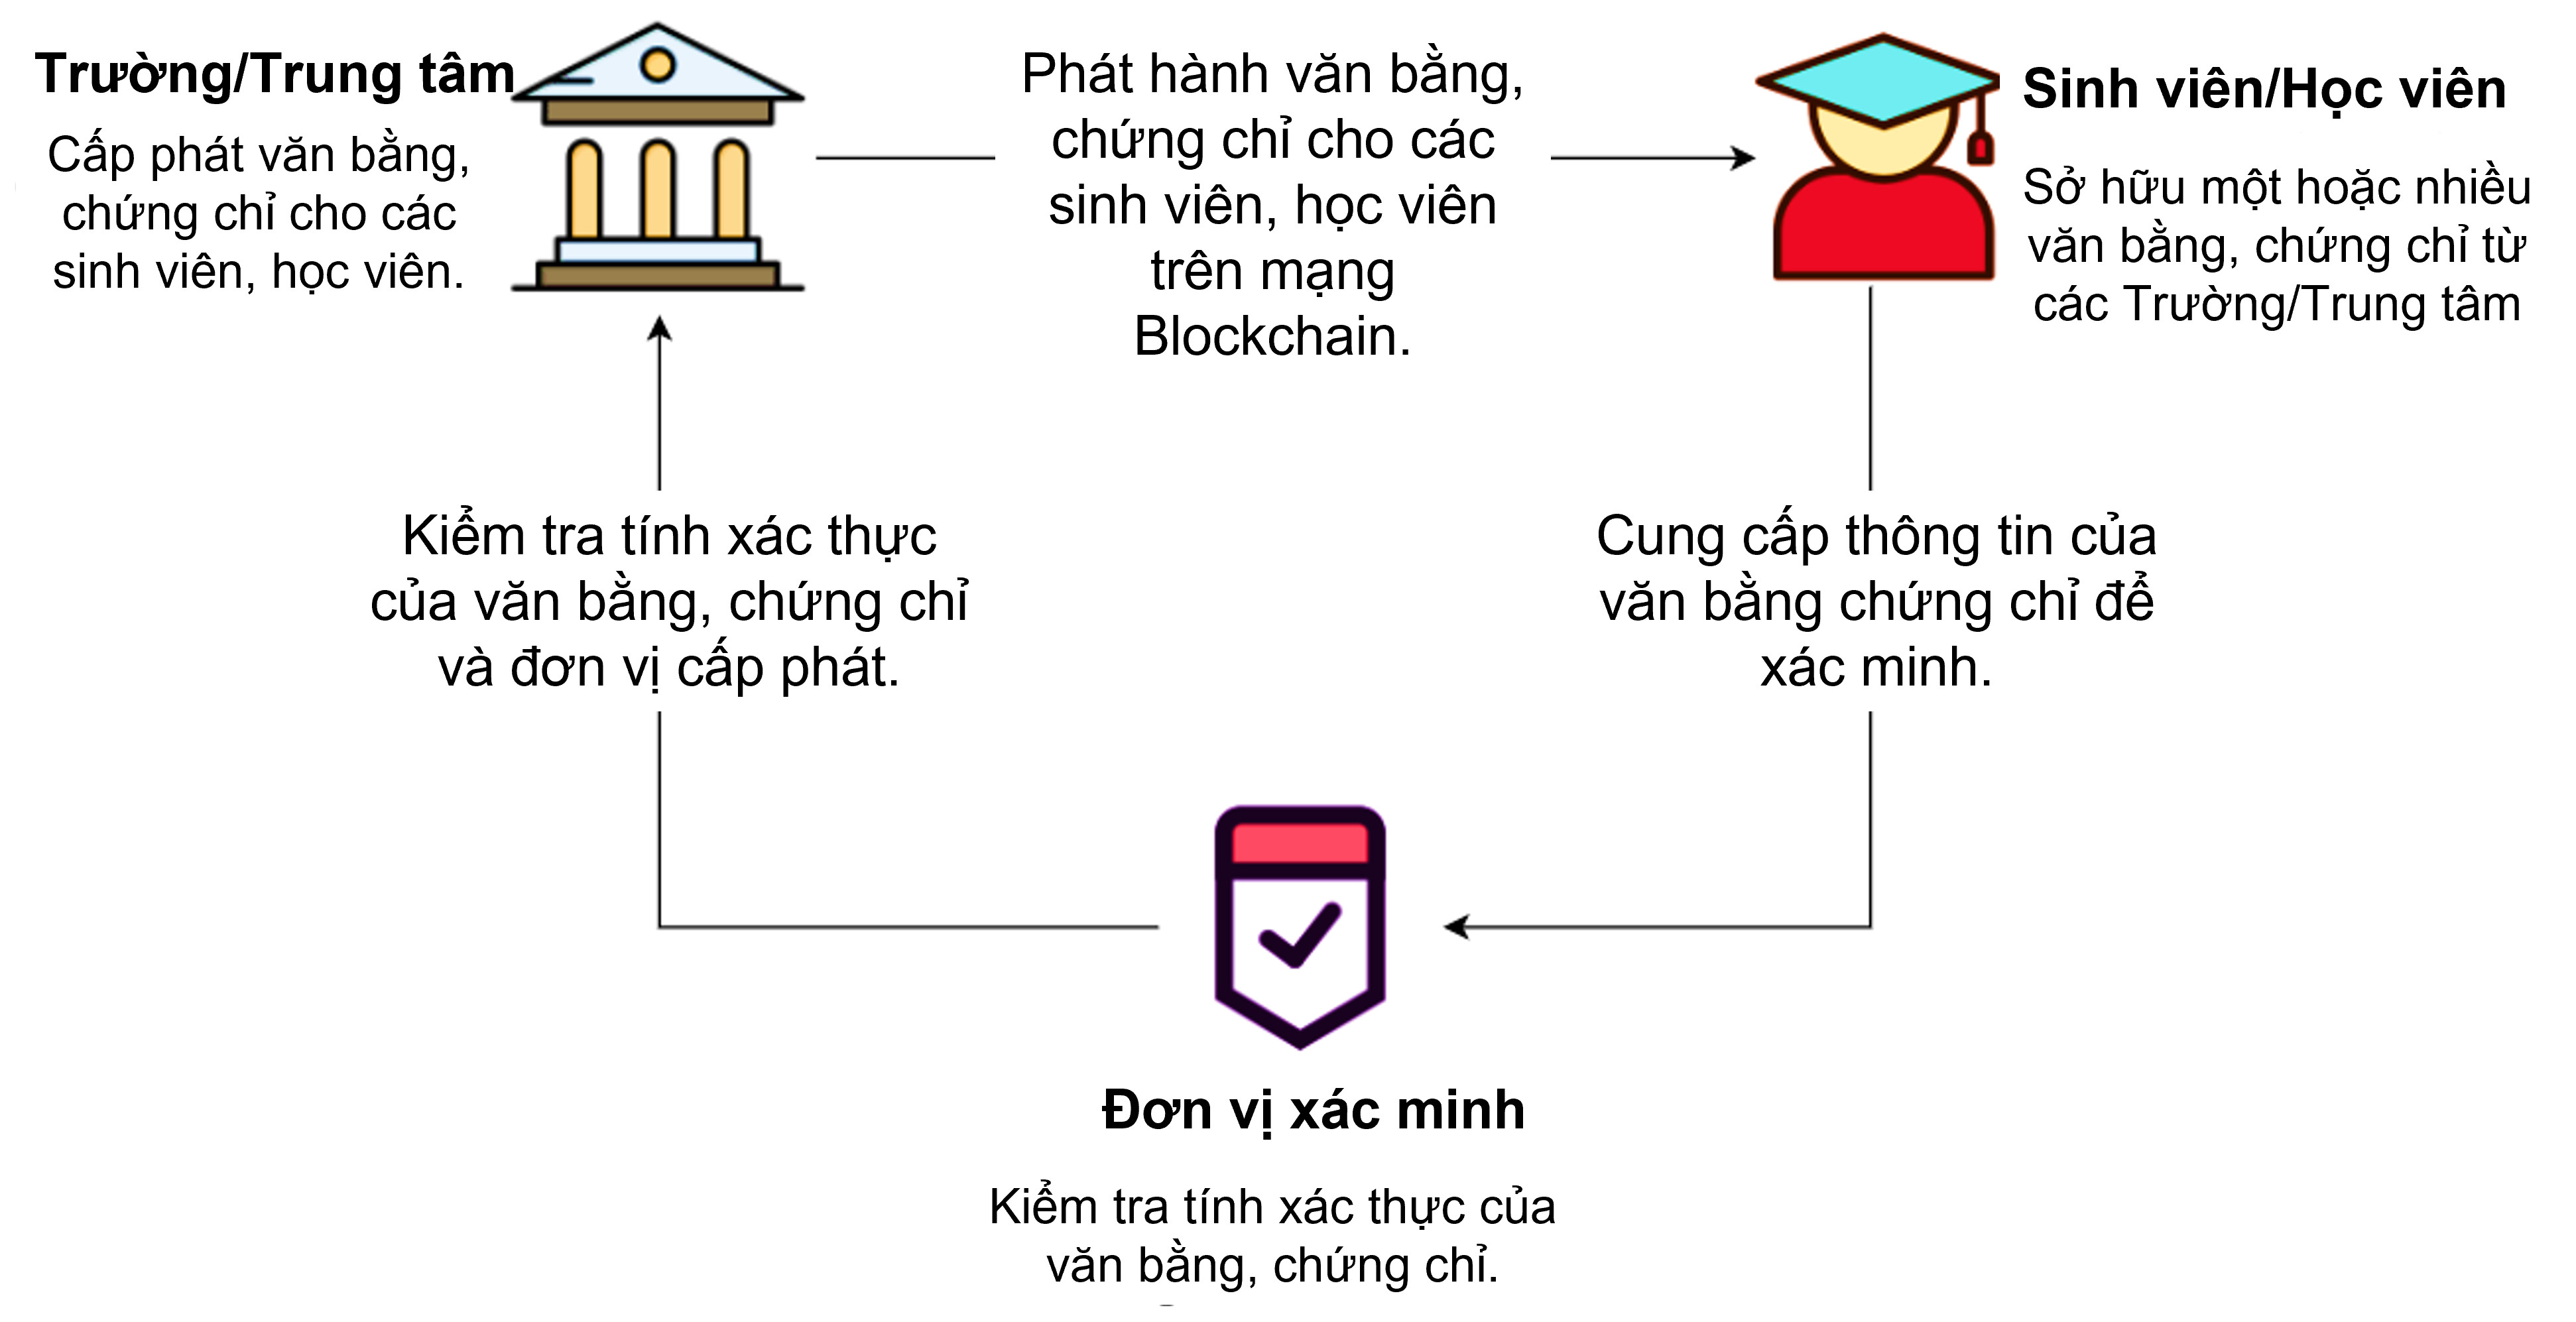
\includegraphics[width=.9\linewidth]{img/vbcc.jpg}
\caption{Sơ đồ bài toán quản lý VBCC}
\label{fig:vbcc}
\end{figure}

{\color{red} Todo: Cần phải diễn giải quy trình quản lý theo hình  \ref{fig:vbcc}}

\section{Tổng quan giải pháp}

Nghiên cứu đề xuất một mô hình thử nghiệm ứng dụng Blockchain để đảm bảo tính an toàn thông tin VBCC và tính bí mật thông tin của người được cấp VBCC.
Hệ thống thực hiện việc ký số khi cấp VBCC, lưu VBCC đã cấp vào blockchain và truy vấn dữ liệu blockchain để xác thực VBCC. 
Kiến trúc hệ thống được mô tả như hình \ref{fig:vbcc_phanmem}.

\begin{figure}[htbp]
\centering
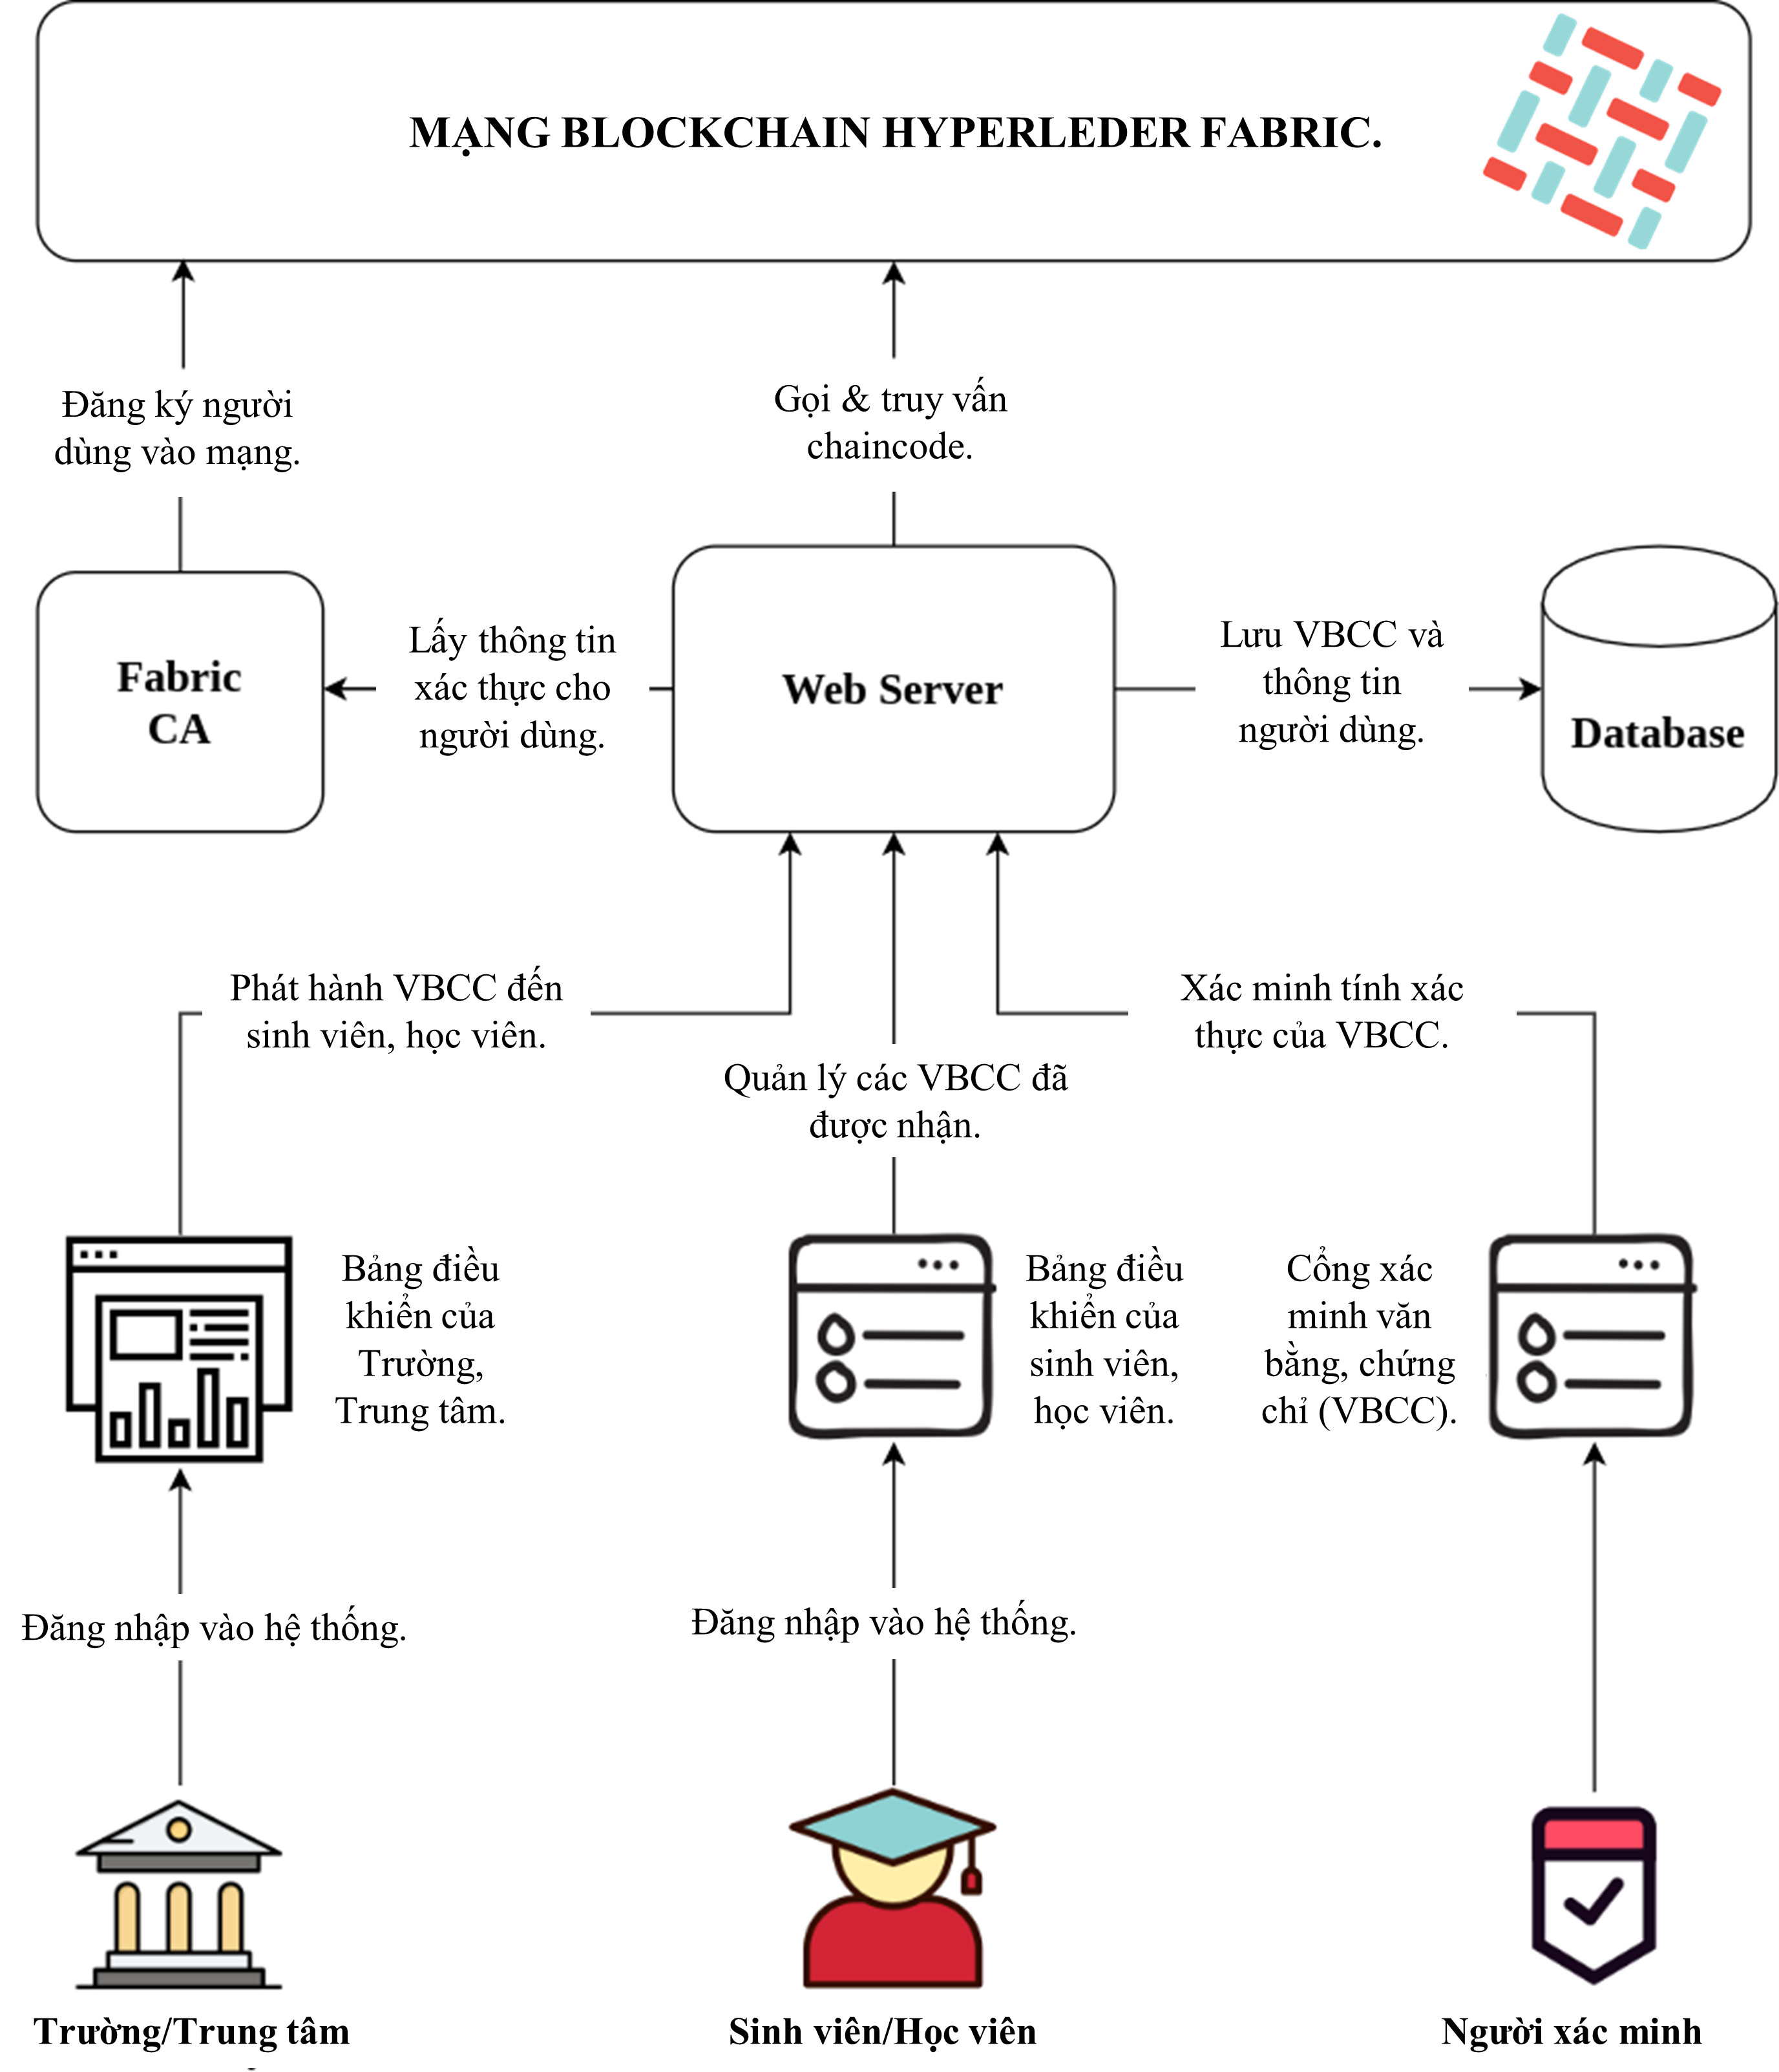
\includegraphics[width=.9\linewidth]{img/vbcc_phanmem.jpg}
\caption{Sơ đồ kiến trúc hệ thống}
\label{fig:vbcc_phanmem}
\end{figure}

{\color{red} Todo: bổ sung diễn giải thêm về các bước hoạt động \ref{fig:vbcc_phanmem}}

Quy trình hoạt động của hệ thống được minh họa như hình \ref{fig:vbcc_diagram}.

\begin{figure}[htbp]
\centering
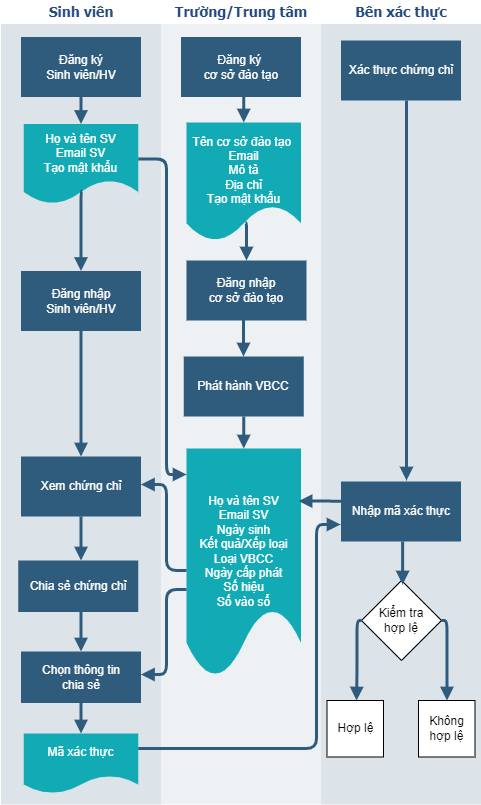
\includegraphics[width=.9\linewidth]{img/vbcc_diagram2.png}
\caption{Quy trình hoạt động của hệ thống}
\label{fig:vbcc_diagram}
\end{figure}

{\color{red} Todo: bổ sung tên bước và diễn giải thêm về các bước quy trình hoạt động \ref{fig:vbcc_diagram}.}

\subsection{Danh sách tác nhân}

\begin{table}[H]
\caption{Danh sách tác nhân}
	\label{table:actor}
	\begin{tabularx} {\textwidth} {|p{1cm}|p{3cm}|X|}
\hline
	ID & Tên actor & Mô tả \\ \hline
	A1 & Sinh viên &  là sinh viên/học viên nhận VBCC \\ \hline
	A2 & Trường học  & Trường/Đơn vị có quyền cấp VBCC \\ \hline
	A3 & Người xác minh  & Người/Đơn vị có nhu cầu xác minh VBCC \\ \hline
\end{tabularx}
\end{table}

\subsection{Danh sách chức năng}

\begin{table}[H]
\caption{Danh sách chức năng}
	\label{table:usecase}
	\begin{tabularx} {\textwidth} {|p{1cm}|p{1cm}|p{3cm}|X|X|}
\hline
		STT &	ID & Tên Use Case & Mô tả & Yêu cầu nghiệp vụ \\ \hline
		1 & U1	& Đăng nhập &Đăng nhập vào hệ thống để xác thực người dùng &Được mở rộng bởi tất cả \\ \hline
		2 & U2 & Đăng ký  & Đăng ký tài khoản vào hệ thống & Được mở rộng bởi tất cả\\ \hline
		3 & U3	&Cấp VBCC & Cấp VBCC có xác nhận chứng thực và ký số VBCC & \\ \hline
		4& U4	& Xem VBCC đã cấp&  Xem các VBCC Trường cấp & \\ \hline
		5 & U5	&Xem VBCC đã nhận & Xem VBCC sinh viên đã nhận& \\ \hline
	6	& U6	&Chia sẻ thông tin VBCC &Chia sẻ thông tin VBCC & \\ \hline
		7& U7	& Xác thực VBCC &Xác minh tính xác thực của VBCC với nền tảng blockchain & \\ \hline
\end{tabularx}
\end{table}

\subsection{Mô tả chức năng hệ thống}
\begin{enumerate}
\item 
Chức năng Đăng ký tài khoản
\begin{itemize}
\item Mô tả: chức năng này cho phép người dùng đăng ký tài khoản để đăng nhập vào hệ thống, để sử dụng các chức năng yêu cầu bắt buộc đăng nhập.
\item Tác nhân: sinh viên, trường cấp VBCC 
\item Yêu cầu: người dùng đã truy cập vào hệ thống 
\end{itemize}

\item 
Chức năng Đăng nhập
\begin{itemize}
\item Mô tả: chức năng để người sử dụng đăng nhập vào hệ thống
\item Tác nhân: sinh viên, trường cấp VBCC
\item Yêu cầu: người dùng đã truy cập vào cập hệ thống
\end{itemize}

\item 
Chức năng Cấp VBCC
\begin{itemize}
\item Mô tả: chức năng cho phép Trường thêm mới một VBCC 
\item Tác nhân: Trường cấp VBCC
\item Yêu cầu: người dùng đã đăng nhập vào hệ thống; người dùng chọn chức năng cấp VBCC
\end{itemize}

\item 
Chức năng Xem VBCC đã cấp
\begin{itemize}
\item Mô tả: chức năng cho phép người dùng xem VBCC đã cấp 
\item Tác nhân: Trường cấp VBCC 
\item Yêu cầu: người dùng đã đăng nhập vào hệ thống; người dùng chọn chức năng xem VBCC
\end{itemize}

\item 
Chức năng Xem VBCC đã nhận
\begin{itemize}
\item Mô tả: chức năng cho phép người dùng xem VBCC 
\item Tác nhân: sinh viên
\item Yêu cầu: người dùng đã đăng nhập vào hệ thống; người dùng chọn chức năng xem VBCC
\end{itemize}

\item 
Chức năng Chia sẻ thông tin VBCC
\begin{itemize}
\item Mô tả: chức năng cho phép người dùng chia sẽ thông tin VBCC 
\item Tác nhân: sinh viên 
\item Yêu cầu: người dùng đã đăng nhập vào hệ thống; người dùng chọn chức năng chia sẽ VBCC
\end{itemize}

\item 
Chức năng Xác thực VBCC
\begin{itemize}
\item Mô tả: chức năng cho phép người dùng xác thực VBCC
\item Tác nhân: người xác minh, sinh viên, trường 
\item Yêu cầu: người dùng truy cập vào hệ thống; người dùng chọn chức năng xác thực VBCC
\end{itemize}

\end{enumerate}

\subsection{Thiết kế CSDL}

Danh sách cấu trúc dữ liệu trong hệ thống

{\color{red} Todo: Bổ sung diễn giải các trường trong từng bảng}

\begin{table}[H]
\caption{Danh sách cấu trúc dữ liệu trong hệ thống}
	\label{table:dataschema}
	\begin{tabularx} {\textwidth} {|p{1cm}|p{3cm}|X|}
\hline
		STT &	Tên cấu trúc & Diễn giải \\ \hline
		1 & certificate	& Cấu trúc thông tin VBCC\\ \hline
		2 & student & Cấu trúc thông tin sinh viên \\ \hline
		3 & university	&Cấu trúc thông tin trường/trung tâm \\ \hline
	\end{tabularx}
\end{table}

Thuộc tính của các cấu trúc dữ liệu

\begin{table}[H]
\caption{Bảng mô tả các thuộc tính của cấu trúc certificate}
	\label{table:certificate}
	\begin{tabularx} {\textwidth} {|p{1cm}|p{3cm}|p{3cm}|X|p{2cm}|}
\hline
		STT &	Tên trường & Kiểu dữ liệu & Diễn giải & Ràng buộc \\ \hline
		1 & studentName	& String & Họ tên  & not null \\ \hline
		2 & studentEmail & String  & Email   & not null \\ \hline
		3 & studentID	&  String & Mã số  & \\ \hline
		4 & birthday	& String & Ngày sinh & \\ \hline
		5 & place	& String & Nơi sinh & \\ \hline
		6 & gender & String & Giới tính & \\ \hline
		7& ethnic	& String & Dân tộc & \\ \hline
		8& universityName	& String & Tên trường cấp VBCC & not null \\ \hline
		9& universityEmail	& String & Email trường cấp VBCC&\\ \hline
		10& major 	& String & Khóa  học  & not null\\ \hline
		11& number	& String & Số hiệu VBCC & not null\\ \hline
		12& regNo	& String & Số vào sổ gốc & not null \\ \hline
		13& departmentName	& String & Tên khoa &\\ \hline
		14& cgpa	& String & Kết quả & not null \\  \hline
		15& dateOfIssuing	& String & Ngày cấp &\\ \hline
		
\end{tabularx}
\end{table}


\begin{table}[H]
\caption{Bảng mô tả các thuộc tính của cấu trúc student}
	\label{table:student}
	\begin{tabularx} {\textwidth} {|p{1cm}|p{3cm}|p{3cm}|X|p{2cm}|}
\hline
		STT &	Tên trường & Kiểu dữ liệu & Diễn giải & Ràng buộc \\ \hline
		1 & email	& String & Email  & not null \\ \hline
		2 & name & String  & Họ tên   & not null \\ \hline
		3 & password	&  String & Mật khẩu  & \\ \hline
		4 & publicKey	& String & Khóa công khai  & \\ \hline
\end{tabularx}
\end{table}


\begin{table}[H]
\caption{Bảng mô tả các thuộc tính của cấu trúc university}
	\label{table:university}
	\begin{tabularx} {\textwidth} {|p{1cm}|p{3cm}|p{3cm}|X|p{2cm}|}
\hline
		STT &	Tên trường & Kiểu dữ liệu & Diễn giải & Ràng buộc \\ \hline
		1 & email	& String & Email  & not null \\ \hline
		2 & name & String  & Tên trường   & not null \\ \hline
		3 & location	&  String & Địa chỉ  & \\ \hline
		4 & password	& String & Mật khẩu  & \\ \hline
		5 & publicKey	& String & Khóa công khai   & \\ \hline
\end{tabularx}
\end{table}

\subsection{Thiết kế blockchain}
\begin{enumerate}
\item 
Danh sách các đối tượng trong hệ thống

{\color{red} Todo: trình bày phần này theo đúng thiết kế theo chuẩn blockchain: blockchain participant, asset, chaincode....}

\begin{table}[H]
\caption{Danh sách các đối tượng trong hệ thống}
	\label{table:asset}
	\begin{tabularx} {\textwidth} {|p{1cm}|p{3cm}|X|}
\hline
		STT &	Tên cấu trúc &  Diễn giải \\ \hline
		1 & certificate	& Chứng chỉ  \\ \hline
		2 & schema  &  Loại VBCC  \\ \hline
		3 & university	&  Trường cấp VBCC  \\ \hline
\end{tabularx}
\end{table}

\begin{table}[H]
\caption{Bảng mô tả các thuộc tính của đối tượng certificate}
	\label{table:assetcertificate}
	\begin{tabularx} {\textwidth} {|p{0.8cm}|p{3.5cm}|p{2.5cm}|X|p{2cm}|}
\hline
		STT &	Tên trường & Kiểu dữ liệu & Diễn giải & Ràng buộc \\ \hline
		1 & certHash	& String & Lưu giá trị băm của VBCC  & not null \\ \hline
		2 & universitySignature & String  & Chữ ký số lên certHash dùng khóa cá nhân của Trường cấp VBCC  & not null \\ \hline
		3 & studentSignature	&  String & Chữ ký số lên certHash dùng khóa cá nhân của sinh viên nhận VBCC  & \\ \hline
		4 & dateOfIssuing	& String & Ngày cấp  & \\ \hline
		5 & certNumber	& String & Số hiệu VBCC  & \\ \hline
		6 & certRegNo	& String & Số vào sổ gốc  & \\ \hline
		7 & certNumber	& String & Số hiệu VBCC  & \\ \hline
		8 & certUUID	& String & Mã số VBCC  & \\ \hline
		9 & universityPK	& String & Khóa công khai của Trường cấp VBCC  & \\ \hline
		10 & studentPK	& String & Khóa công khai của sinh viên nhận VBCC  & \\ \hline
\end{tabularx}
\end{table}


\begin{table}[H]
\caption{Bảng mô tả các thuộc tính của đối tượng schema}
	\label{table:assetschema}
	\begin{tabularx} {\textwidth} {|p{1cm}|p{3cm}|p{3cm}|X|p{2cm}|}
\hline
		STT &	Tên trường & Kiểu dữ liệu & Diễn giải & Ràng buộc \\ \hline
		1 & certificateType	& String & Loại VBCC  & not null \\ \hline
		2 & id  & String  & Mã loại  & not null \\ \hline
		3 & ordering	&  String &   & \\ \hline
	\end{tabularx}
\end{table}


\begin{table}[H]
\caption{Bảng mô tả các thuộc tính của đối tượng university}
	\label{table:assetuniversity}
	\begin{tabularx} {\textwidth} {|p{1cm}|p{3cm}|p{3cm}|X|p{2cm}|}
\hline
		STT &	Tên trường & Kiểu dữ liệu & Diễn giải & Ràng buộc \\ \hline
		1 & name	& String & Tên Trường cấp VBCC  & not null \\ \hline
		2 & publicKey & String  & Khóa công khai của Trường cấp VBCC  & not null \\ \hline
		3 & location	&  String & Địa điểm  & \\ \hline
		4 & description	& String & Thông tin mô tả  & \\ \hline
\end{tabularx}
\end{table}

\end{enumerate}
